\chapter{Liquid Argon Detectors at the Intensity Frontier}\label{ch:2}
In the next few years, LArTPCs will  be the tools to answer some of the burning questions in neutrino physics today.  This section illustrates the operational principles of this detector technology, as well as the scope of the key detectors in the US liquid argon program -- SBN, DUNE and LArIAT.


\section{The Liquid Argon Time Projection Chamber Technology}

\subsection{TPCs, Neutrinos \& Argon}
David Nygren designed the first Time Projection Chamber (TPC) in the late 1970s \textcolor{red}{[15]} for the  PEP-4 experiment, a detector  apt to study electron-positron collisions at the PEP storage ring at the SLAC National Accelerator Laboratory.
From the original design  in the seventies -- a cylindrical chamber filled with methane gas -- the TPC detector concept has seen many incarnations, the employment of several different active media and a variety of different particle physics applications, including, but not limited to the study of electron/positron storage rings (e.g. PEP4, TOPAZ, ALEPH and DELPHI), heavy ions collisions in fixed target and collider experiments (e.g. EOS/HISS and ALICE ), dark matter (ArDM), rare decays and capture (e.g. TRIUMP, MuCap),  neutrino detectors and nucleon decay (ICARUS, SBN, DUNE), and neutrino less double beta decay (Next). A nice review of the history of TPCs and working principles is provided in \cite{0034-4885-73-11-116201}.

Several features of the TPC technology make these detectors a more versatile tool compared to other ionization detectors and explain such a wide popularity. TPCs are the only electronically read detector which deliver simultaneous  three-dimensional track information and a measurement of the particle energy loss. Leveraging on both tracking and calorimetry,  particle identification (PID) capabilities are enhanced  over a wide momentum range.

Carlo Rubbia first proposed the use of a Liquid Argon TPC for a neutrino experiment, ICARUS \textcolor{red}{[14]}, in 1977. The active medium in ionization detector has historically been in the gaseous form. Nevertheless, using nobles elements in the liquid form for neutrino detectors is advantageous for several reasons.  The density of liquids is $\sim$1000 times greater than gases, increasing the number of target centers for neutrino's interaction in the same volume. Since the energy loss of charged particle is proportional to the target material density, as shown in the Bethe-Block equation in \ref{eq:BB}, the increased density reflects into a proportionally higher energy loss, enhancing the calorimetry capability of detectors with a liquid active medium. Additionally, the ionization energy of liquids is smaller than gasses by the order of tens of eV. Thus, at the passage of charged particles, liquid generally produce more ionization electrons than gas for the same deposited energy and force the particles to deposit more energy in a shorter range. The downside of using noble liquid gasses in experiments is that they require a cryogenic system to cool the gas until it transitions to its the liquid form.
The properties of liquid argon in comparison liquid xenon -- a popular choice for dark matter and neutrinoless double beta decay detectors -- are summarized in table \ref{tab:properties}.  Albeit xenon would be more desirable than argon given some superior properties such as lower ionization energy and higher density and light yield, argon relative abundance abates the cost of argon compared to xenon, making argon a more viable choice for the construction of big neutrino detectors. 




\begin{table}[]
\centering
\begin{tabular}{|l|c|c|}\hline
Element & LAr & LXe \\
\hline
\hline
Atomic Number &  18 &54 \\
Atomic weight A & 40  & 131\\
Boiling Point Tb at 1 atm & 87.3 K & 165.0 K\\
Density  & 1.4 g/cm$^3$& 3.0 g/cm$^3$\\
Radiation length  & 14.0 cm& 2.8 cm \\
Moliere Radius  &10.0 cm& 5.7 cm\\
Work function  & 23.6 eV&15.6 eV\\
Electron Mobility at $E_{field} =10^4$ V/m &0.047 m$^2$/Vs& 0.22 m$^2$/Vs\\
Average dE/dx MIP  & 2.1 MeV/cm&3.8 MeV/cm\\
Average Scintillation Light Yield & 40000 $\gamma$/MeV&42000 $\gamma$/MeV\\
Scintillation $\lambda$  &128 nm&175 nm\\
\hline
\end{tabular}
\caption{LAr, LXe summary of properties relevant for neutrino detectors.}
\label{tab:properties}
\end{table}


LArTPCs are some times referred as to ``electronic" bubble-chambers, for the similarity in the tracking and energy resolution which is coupled with an electronic readout of the imaging information in LArTPCs. Compared to these historic detectors however, LArTPC bestow tridimensional tracking and a self triggering mechanism provided by the scintillation light in the noble gas.  A comparison between a neutrino interaction in the ArgoNeut LArTPC and in the bubble chamber is shown in picture \textcolor{red}{EVENT DISPLAY}. 


\subsection{LArTPC: Principles of Operation}\label{sec:LArTPCWorkingPrinciple}

%The time projection chamber (TPC) was invented by Nygren in 1974 [91]. The proposal to implement a liquid argon TPC (LArTPC) for neutrino physics was made by Rubbia in 1977 [92], and the concept was implemented by the ICARUS collaboration [93]. 

To the bare bones, a LArTPC is a bulk of liquid argon sandwiched in a flat capacitor, equipped with a light collection system. A uniform electric field of the order of 500 V/cm is maintained constant between the faces of the capacitor. The anode is sensitive to ionization charge and it is usually made of two or more planes segmented into several hundreds parallel sense wires a few millimeters apart; different geometries for the anode segmentation are under study \cite{1748-0221-8-07-P07002}. 

Argon ionization and scintillation are the processes leveraged to detect particles in the LArTPC active volume.  When a ionizing radiation traverses the argon active volume it leaves a trail of ionization electrons along its trajectory and it excites the argon, leading to the production of scintillation light -- details on the production and detection of ionization charge and scintillation light are provided in \ref{sec:light} and \ref{sec:light} respectively. The optical part of the detector collects the argon scintillation light in matters of nanoseconds. This flash of light determines the start time of an event in the chamber, $t_0$. The uniform electric field drifts the ionization  electrons from the production point towards the anode plane in order of hundreds of microseconds or more depending on the chamber dimensions\footnote{The ionized argon also drifts, but  in the opposite directions compared to the electrons. Since the drift time is proportional to the particle mass,  the ions drift time is much longer than the electrons'.  Ionized argon is collected on the cathode which is not instrumented, so it is not used to infer information about the interactions in the chamber.}. The anode sense wires see either an induced current by the drifting charge (on induction planes) or an injection of the ionization charge (collection plane) \textcolor{red}{[94]}.    An appropriate choice of the voltage bias on each wire plane assures ideal charge transparency, so that all the ionization charge is collected on the collection plane and none on the induction planes \textcolor{red}{[95]}.  

The arrival time of the charge on the anode sense wires is used to measure the position of the original ionizing radiation in the drift direction. In fact, since the constant electric field implies that the drift velocity is also constant in the chamber, the position of the original ionization is simply given by the multiplication of the drift velocity by the drift time, where we define as ``drift time" the difference between $t_0$ and the charge arrival time on the wire planes. The spacial resolution on this dimension is limited by the time resolution of the electronics or by longitudinal diffusion of the electrons.
The spatial information on the different wire planes maps a bi-dimensional projection of the interaction pattern in the plane perpendicular to the drift direction. The spacial resolution on this dimension is limited by the transverse electron diffusion in argon and by the grain of the anode segmentation, i.e. the spacing between the wires in the sense planes \textcolor{red}{[100]}.  The off-line combination of the 2-D information on the wire planes with the timing information allows for the 3D reconstruction of the event in the chamber.

Since the charge deposited by the ionizing radiation in the chamber is proportional to the deposited energy and the charge collected on the sense plane is a function of the deposited charge, LArTPC allow the measurement of the energy deposit in the active volume. Effects due to the presence of free charge and impurities in the active volume, such as a finite electron lifetime, recombination and space charge, complicate the relationship between deposited and collected charge affecting the measurement of the particle's energy, as described in the next section.
 
\subsection{Liquid Argon: Ionization Charge}\label{sec:charge}

\begin{eqnarray*}
			- \frac{dE}{dx} = K z^2 \frac{Z}{A} \varrho \frac{1}{\beta^2} \left[ \frac{1}{2} \ln{\frac{2 m_e c^2 \beta^2 \gamma^2 T_{max}}{I^2}} - \beta^2 - \frac{\delta}{2}\right] 
			\label{eq:BB}
		\end{eqnarray*}
		
\subsubsection{Purity \& Electron Life Time }
The presence of electronegative contaminants in liquid argon, such as oxygen and water, is particularly
pernicious, since these molecules quench the charge produced by the ionizing radiation.  Thus, amount of charge per unit of length $dQ/dx$ collected on the collection plane depends on the charge's production point in the detector: a ionization produced  close to the cathode will see more impurities along its journey to the collection plane than ionization produced close to the anode, resulting in greater attenuation. As a result,  the amount of charge collected on the sense wires as a function of the traveled distance follows an exponential decay trend. The traveled distance is generally measured in terms of drift time and the  characteristic time constant of the exponential decay is called electron lifetime $\tau_e$. Figure \ref{fig:Elifetime} shows the typical life time for LArIAT data \textcolor{red}{cite technote}. LArIAT small drift distance (47 cm) allows for a relatively short electron life time. The life time for bigger detectors such as MicroBooNE, whose drift distance is 2.5 m, needs to be of the order of  to allow charge collection usable for physics analyses. Energy reconstruction in LArTPC applies a correction for the finite lifetime to calibrate the detector calorimetric response; details for LArIAT are provided in Section \ref{ch:energyCalibration}.

LArTPCs use  hermetically sealed and leak-checked vessels to abate the leakage and diffusion of contaminants into the system. The liquid argon filling of the volume occurs after the vessel is evacuated or purged with gaseous argon \textcolor{red}{[205]} to reduce remaining gases in the volume. Even so, the construction of a pure tank of argon is unviable, as several sources of impurity remain.  In particular, impurities can come from the raw argon supply, the argon filtration system and from the outgassing from internal surfaces. Outgassing is a continuous diffusive process  producing contaminants, especially water, even after the vessel is sealed, particularly from materials in the ullage region\footnote{.  While the liquid argon low temperature reduces outgassing in the liquid, this process remains significant for absorptive material (such as plastic) above the surface of the liquid phase}.  Since research-grade argon comes from the industrial distillation of air, the impurities with the highest concentration are nitrogen, oxygen and water, generally maintained under the 1 part per million level by the vendor.  Even so, a higher level of purity is necessary to achieve a free electron life time usable in meter scale detectors. Thus, argon  is constantly  filtered in the cryogenic system, which reduce the oxygen and water contamination to less than 100 parts per trillion. The filtration system depends on the size and drift distance of the experiment and, for experiments on several meters scale, it includes an argon recirculation system.

%% Life time value for LArIAT


\subsubsection{Recombination Effect}
After production, ionization electrons thermalize with the surrounding medium and may recombine with nearby ions. Recombination might occur either between the electron and the parent ion through Coulomb attraction (Onsager geminate theory  [2] ) or thanks to the collective charge density of electrons and ions from multiple ionizations in a cylindrical volume surrounding the particle trajectory (Jaffe[3]  columnar model ). 
Consideration on the  average electron-ion distance and the average ion-ion distance for argon show that the probability of geminate recombination is low; thus recombination in argon is mainly due to collective effects\cite{1748-0221-8-08-P08005}.  Since protons, kaons and stopping particles present a higher ionization compared to MIPs, recombination effects are more prominent when considering the reconstruction of energy deposited by these particles.

Models for a theoretical descriptions of recombination base on are provided in (Birks model [6]) and in (Box model [7]). The Birks model assumes a gaussian spatial distribution around the particle trajectory during the entire recombination phase and identical charge mobility for ions and electrons. The Box model also assumes that electron diffusion and ion mobility are negligible in liquid argon during recombination
In these models, the fraction of ionization electrons surviving recombination is a function of the number of ion-electron pairs per unit length, the electric field, the average ion-electron separation distance after thermalization and the angle of the particle with respect to the direction of the electric field -- plus the diffusion coefficient in the Birks model. Given the stringent assumptions, it is perhaps  not surprising that these models are in accordance to data only in specific regimes: the Birks model is generally used to describe recombination for low dE/dx, the Box model for high dEdX.
In LArTPC, the ICARUS and ArgoNeut have measured recombination in [8] and \cite{1748-0221-8-08-P08005} respetively. Since LArIAT uses the refurbished ArgoNeut TPC and cryostat,  LArIAT currently corrects for recombination using the ArgoNeut measurement, shown in figure \textcolor{red}{find figure}.


\subsubsection{Space Charge Effect}
Slow-moving positive argon ions created during ionization can build-up in LArTPC, causing the distortion of the
electric field within the detector. This effect, called  ``space charge effect" leads to a displacement in the reconstructed position of the signal ionization electrons. In surface LArTPCs the space charge effect is primarily due to the rate of ionization produced by cosmic rays which is slowly drifting in the chamber at all times. Surface LArTPC of the size of several meters are expected to be modestly impacted from the space charge effect, where charge build-up create anisotropy of the electric field magnitude of the order of  5\% at a drift field of 500 V/cm. The smallness of the LArIAT drift volume is such that  effect of  space charge on the electric field is expected to b even smaller. \textcolor{red}{CHIEDI A FLAVIO}

%%%%%%%%%%%%%%%%%%%%%%%%%%%%%%%%%%%%%%%%%%%%%%%%%%%%%%%%%%%%%%%
%%%%%%%%%%%%%%%%%%%%%                     Light Detection             %%%%%%%%%%%%%%%%%%%%%%%%
%%%%%%%%%%%%%%%%%%%%%%%%%%%%%%%%%%%%%%%%%%%%%%%%%%%%%%%%%%%%%%%
\subsection{Liquid Argon: Scintillation Light }\label{sec:light}
Liquid argon emits scintillation light at the passage of charged particles. LArTPCs  leverage this property to determine when the ionization charge begins to drift towards the anode plane. %Scintillation light can also be used for particle identification, as discussed in the next sections.

\subsubsection{Scintillation Process}
Scintillation light in argon peaks in the ultraviolet at a 128 nm, shown in comparison to Xenon and Kypton in Figure  \textcolor{red}{[183]}. The light yield collected by the optical detector depends on the argon purity, the electric field, the dE/dx and particle type, averaging at the tens of thousands of photons per MeV. 
The de-excitation of Rydberg dimers in the argon is responsible for the scintillation light. 
Rydberg dimers exist in two states:  singlets and a triplets. The time constant for the singlet radiative decay is 6 ns, resulting in a prompt component for the scintillation light. The decay of the triplet is delayed by intersystem crossing, producing a slow component with a time constant of $\sim$~1500 ns.  ``Self-trapped exciton luminescence" and  ``recombination luminescence" are the two processes responsible for the creation of the Rydberg dimers. In the first process, a charged particle excites an argon atom which becomes self-trapped in the surrounding bulk of argon,  forming a dimer; the dimer is in the singlet state 65\% of the times and in the triplet state 35\% of the times. In case of recombination luminescence, the charged particle transfers enough energy to ionize the argon. The argon ion forms a charged argon dimer state, which quickly recombines with the thermalized free electron cloud. Excimer states are produced in the recombination, roughly half in the singlet and half in the triplet state. The light yield dependency on the electric field, on the dE/dx and particle type derives from the role of free charge in the recombination luminescence process. The spacial separation between the argon ions and the free electron cloud depends on the electric field. On one hand, a strong electric field diminishes the recombination probability, leading to a smaller light yield; on the other, it increases the free charge drifting towards the anode plane. Hence, the amount of  measurable charge and light anti-correlates as a function of the electric field.  Ionizing particles in the argon modify the local density of both free electrons and ions depending on their dE/dx. Since the recombination rate is proportional to the square of the local ionization density, highly ionizing particles boost recombination and the subsequent light yield compared to MIPs.  The possibility to leverage this dependency for pulseshape-based particle identification has been shown in \textcolor{red}{[186], [187]}.

\subsubsection{Effects Modifying the  Light Yield}
The production mechanism through emission from bound excimer states implies that argon is  transparent to its own scintillation light. In fact, the photons emitted from these metastable states are not energetic enough to re-excite the argon bulk, greatly suppressing absorption mechanisms. In a LArTPC however, several processes modify the light yield in between the location where light is produced and the optical detector. In a hypothetical pure tank of argon, Rayleigh scattering would be the most important processes modifying the light yield. Rayleigh scattering changes the path of light propagation in argon, prolonging the time between light production and detection.  The scattering length has been measured to be 66 cm \textcolor{red}{[191]} , shorter than the theoretical prediction of $\sim$~90 cm \textcolor{red}{[190]}; this value is short enough to be relevant for the current size of LArTPCs detectors. In fact, Rayleigh scattering worsen the resolution on $t_0$, the start time for charge drifting, and  alters the light directionality, complicating the matching between light and charge coming from the same object in case of multiple charged particles in the detector. 

Traces of impurities in argon such as oxygen, water and nitrogen  also affect the light yield, mainly  via absorption and quenching mechanisms. 
Absorption occurs as the interaction of a 128 nm photon directly with the impurity dissolved in the liquid argon.  Differently, quenching occurs as the interaction of an argon excimer and an impurity, where the excimer transfers its excitation to the impurity and  dissociates non-radiatively.  Given this mechanism, it is evident how quenching is both a function of the impurity concentrations and the excimer lifetime.  Since the triplet states live much longer than the singlet states,  quenching occurs mainly on triplet states, affecting primarily the slow component of the light,  reducing the scintillation yield and a shortening of the scintillation time constants.  

The stringent constraints for the electron life time limit the presence of oxygen and water to such a low level that both absorption and quenching on these impurity is not expected to be significant \textcolor{red}{[210]}.   Contrarily, the nitrogen level is not bound by the electron life time constraints -- nitrogen being an inert gas, expensive to filter. Thus, nitrogen is often present at the level provided by the vendor. The effects of nitrogen on argon scintillation light have been studied in the WArP R\&D program and at several test stands.
The quenching process induced by nitrogen in liquid Ar has been measured to be proportional to the nitrogen concentration, with a rate constant of $\sim  0.11$ $\mu s^{-1}$ ppm$^{-1}$; appreciable decreasing in lifetime and relative amplitude of the slow component have been shown for contamination as high as a few ppm of nitrogen \cite{1748-0221-5-06-P06003}.
For a nitrogen  concentration of 2 parts per million,  typical of the current generation of LArTPC, the attenuation length due to nitrogen has been measured to be $\sim$30 meters \cite{1748-0221-8-07-P07011}. 



\subsubsection{Wavelength Shifting of LAr Scintillation Light}
Liquid argon scintillation light is invisible for most optical detectors deployed in LArTPC, such as cryogenic PMTs and SiPMs, since a wavelength of 128 nm is  generally too short to be absorbed from most in glasses, polymers and semiconductor materials. Research on prototype SiPMs absorbing directly VUV light and their deployment in noble gasses experiment is ongoing but not mature \cite{1748-0221-8-01-C01003}. Thus, experiments need to shift the wavelength of scintillation light to be able to detect it.  Albeit deployed in different ways, neutrinos and dark matter experiments commonly use  1,1,4,4-tetraphenyl-butadiene (TPB) to shift the scintillation light. 
TPB, whose chemical structure is shown in figure , absorbs the vacuum ultraviolet (VUV) light and emits in the visible at $\sim$~425 nm \textcolor{red}{[231]}, with a ratio of visible photon emitted per VUV photon absorbed of $\sim$1.2:1 \cite{GEHMAN2011116}.

Neutrino experiments typically coat their optical detector system evaporating a layer of TPB either directly on the PMTs glass surface or on acrylic plates mounted in front of the PMTs \textcolor{red}{cite microboone}; this technique allows the fast detection light coming directly from the neutrino interaction. Dark matter experiments typically evaporate TPB on reflective foils mounted on the inside walls of the sensitive volume and detect the light after it has been reflected; this technique leads to a higher and more uniform light yield, though scattering effects for both the visible and VUV light augment the propagation time and hinder directionality information\textcolor{red}{some DM detector} . In order to take advantage of both these techniques, hybrid systems with PMT coating and foils are being considered for the next generation of large neutrino detectors \textcolor{red}{cite SBND?}. 

\subsection{Signal Processing and Event Reconstruction}
In this section we illustrate the processing and reconstruction chain of the TPC signals, from the pulses on the sense wire to the construction of three dimensional objects with associated calorimetry.\\

\textbf{Deconvolution.} Induction and collection planes have different field responses, given the different nature of the signals on these planes: the wires on the induction planes see inductive signal of the drifting charge, while the wires on the collection planes see the current derived from the charge entering the conductor. Thus, signals on the induction plane are bi-polar pulse and signal on the collection plane are unipolar pulses, see Figure \textcolor{red}{ADD PULSES FIGURE}. The first step in signal processing is deconvolution, that is a series of off-line algorithms geared towards undoing the detector effects. The result of the deconvolution step is  the production of  a comparable set waveforms on all planes presenting unipolar, approximately gaussian-like pulses. Signal from all planes are treated on equal footage beyond this point. Some LArTPC apply noise filtering in the frequency domain just after the deconvolution to clean up wire cross talk. Since signals from the LArIAT TPC are extremely clean, noise filtering is not necessary.\\


\textbf{Hit Reconstruction.} The second stage of the signal processing is the reconstruction of hits, indicating an energy deposition in the detector.  A peak finder scans the deconvolved TPC waveforms for each wire on the whole readout time looking for spikes  above  the waveform's baseline. It then fits these peaks with gaussian shapes and stores the fit parameters such as the quality of the fit, the peak time, height and area under the gaussian fit. The information resulting fron this process a single spike form a single reconstructed ``hit".
The next steps in the event reconstruction chain will then decide if rejecting hits with poor fits.
It is important to notice how the height and width of the hit depend on the topology of the event: for example, a particle running  parallel to the wire planes will leave a series of sharp hits on many consecutive wires, while a particle traveling towards the planes will leave a long, wide hit on very few wires. The height of the hits and their integral is proportional to the charge collected on the wire, so it depends on the particle type.

The event reconstruction chain uses collection of hits to form more complex objects associated with the particles in the detector. The development of different approaches to accomplish this task is an extremely hot topic in LArTPC event reconstruction which spans from more traditional approaches such as line-clustering  \cite{MicroBooNE} \textcolor{red}{argoneut paper} to the use of machine learning tools \cite{MicroBooNE} \textcolor{red}{KAZU'S paper}. Generally speaking, the scope of hit clustering and event reconstruction to provide shower-like or track like-objects with an associated energy reconstruction. This is because different particles have different topology in the detector -- electrons and photon create electromagnetic showers,  resulting in shower-like topologies, while muons and hadrons  leave track-like signals.  For the scope of these thesis, we will describe only LArIAT's approach to track reconstruction even if we recognize the breath of LArTPC event reconstruction is much wider. We are interested in the reconstruction of pions and kaons in the active volume, whose topology is track-like.\\

\textbf{2D Clustering Reconstruction.} 
The LArIAT reconstruction of track-like objects starts by clustering hits on the collection and induction planes separately with the use of the TrajCluster clustering package\cite{Bruce} \textcolor{red}{Bruce}. 
TrajCluster looks for a collection of hits in the wire-time 2D space which can be described with a line-like 2D trajectory. TrajCluster reconstructs trajectories by adding trajectory points to the leading edge of the trajectory while stepping through the 2D space of hits. Several factors determine whether a hit is added to the trajectory, including but not limited to
\begin{enumerate}
\item the goodness of the fit of the single hit,
\item the charge of the hit compared to the average charge and RMS of the hits already forming the trajectory,
\item the goodness of trajectory fit with and without the hit addition,
\item the angle between the two lines formed by the collection of hits before and after the considered hit in the trajectory.
\end{enumerate}

\textbf{TrackReconstruction.} 

\section{The Intensity Frontier Program}
\subsection{SBN: Neutrino Interaction and Detection}
%\subsection{SBN Goals}
%\subsection{Neutrino Interactions and Detection }
\subsection{DUNE: Rare Decay Searches}
DUNE will achieve a wide non-accelerator physics program.
The key elements for a rare decay experiment are: massive active volume, long exposure, high identification efficiency and low background. 
%The limit to proton lifetime in case of absence of signal and backgrounds is set by calculating
%$$\tau/B > M\times \epsilon\times T \times 10^{32},$$ 
%where M is the detector mass in kton, $\epsilon$ the signal detection efficiency after cuts to suppress backgrounds (dependent on the considered decay mode), T is the exposure in years, B the assumed branching fraction for the considered mode and  $10^{32}$ is a factor accounting for the number of nucleons in a kton of material \cite{Bueno2007}.
Figure \ref{fig:PDKExperimentalLImit} shows the current best experimental limits on nucleon decay lifetime over branching ratio (dots). Historically, the dominant technology used in these searches has been water Cherenkov detectors: all the best experimental limits on every decay mode are indeed set by Super-Kamiokande \cite{PhysRevD.90.072005,PhysRevLett.115.121803}.  It is particularly important to notice that the kaon energy for the proton decay mode $p \rightarrow K^+ \bar{\nu}$ is under Cherenkov threshold.  Super-Kamiokande set the limit on the lifetime for the $p \rightarrow K^+ \bar{\nu}$ mode by  relying exclusively on photons from nuclear de-excitation. For this reason, an attractive alternative approach to identifying nucleon decay is the use of a Liquid Argon Time Projection Chamber (LArTPC). 

LArTPCs can complement nucleon decay searches in modes where water Cherenkov detectors are less sensitive, especially $p\rightarrow K^+\bar{\nu}$. According to \cite{Acciarri:Dune}, DUNE will have an active volume large enough, have sufficient shielding from the surface, and will run for lengths of time sufficient to compete with Hyper-K, opening up the opportunity for the discovery of nucleon decay. 

\begin{figure}[hbpt]
\centering
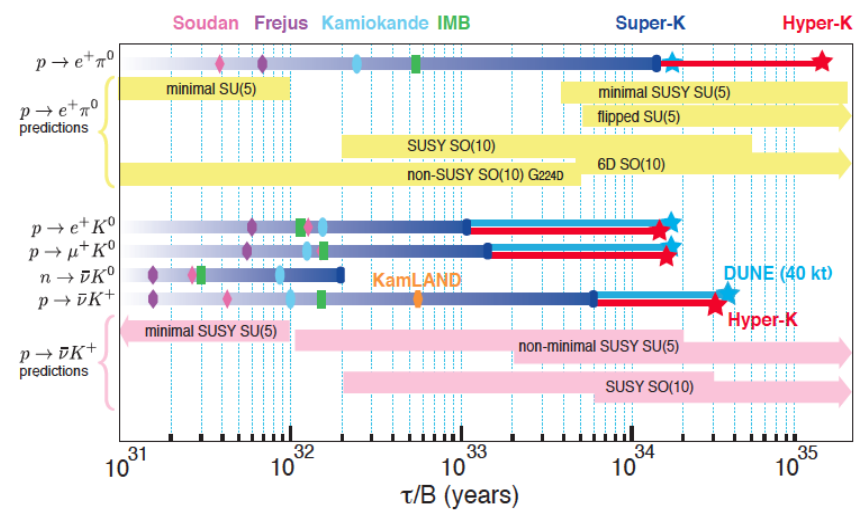
\includegraphics[width=6.5in]{Chapter-2/Images/PDKExperimentalLImit.png}
\caption{Proton decay lifetime limits from passed and future experiments.}
\label{fig:PDKExperimentalLImit}
\end{figure}


\begin{figure}[hbpt]
\centering
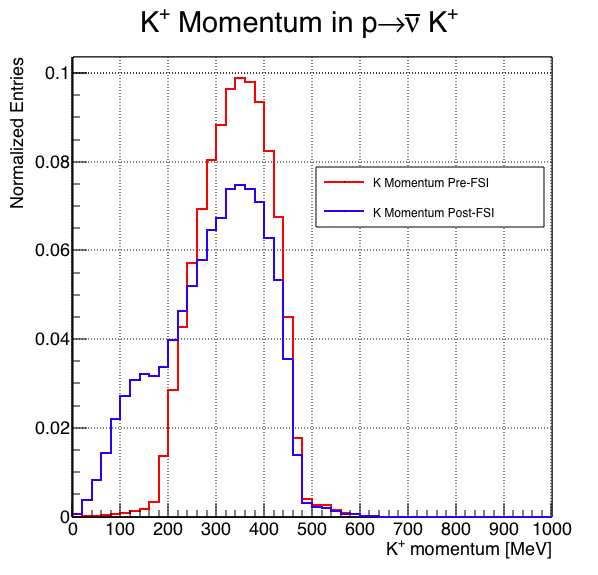
\includegraphics[width=3.5in]{Chapter-2/Images/pdkGenie.png}
\caption{Momentum of the kaon outgoing a proton decay event as simulated by the Genie 2.8.10 event generator in argon. The red line represent the kaon momentum distribution before undergoing the simulated final state interaction inside the argon nucleus, while the blue line represents the momentum distribution after FSI. }
\label{fig:PDKGENIE}
\end{figure}


%\subsection{Non-Accelerator Physics Program}
%\subsection{Rare Decay Searches: Experimental Limit}
%\subsection{Nucleon Decay Detection in LAr}
\subsection{Enabling the next generation of discoveries: LArIAT}
LArIAT, a small Liquid Argon Time Projection Chamber (LArTPC) in a test beam,  is designed to perform an extensive physics campaign centered on charged particle cross section measurements while characterizing the detector performance for future LArTPCs. LArTPC represents one of the most advanced experimental technologies for physics at the Intensity Frontier due to its full 3D-imaging, excellent particle identification and precise calorimetric energy reconstruction. This complex technology however needs a thorough calibration and dedicated measurements of some key quantities to achieve the precision required for the next generation of discoveries at the Intensity Frontier which LArIAT can provide. 

The LArIAT LArTPC is deployed in a dedicated calibration test beamline at Fermilab.
We use the LArIAT beamline to characterize the charge particles before they enter the TPC: the particle type and initial momentum is known from beamline information. The precise calorimetric energy reconstruction of the LArTPC technology enables the measurement of the total differential cross section for  tagged hadrons. 
The Pion-Nucleus and Kaon-Nucleus total hadronic interaction cross section have never been measured before in argon and they are a fundamental step to shed light on light meson interaction in nuclei. Additionally, these measures provides a key input to neutrino physics and proton decay studies in future LArTPC experiments like SBN and DUNE.
\textcolor{red}{add paragraph on all wonderful things lariat can do... some event displays would be nice!}



\textcolor{red}{ADD genie proton decay kaon distribution and lariat beamline overlaied}
The signature of a proton decay event in the ``LAr golden mode" is the presence of a single kaon of about 400 MeV in the detector. 
